\documentclass[a4paper,12pt]{article} % тип документа

% Поля страниц
\usepackage[left=2.5cm,right=2.5cm,
    top=2cm,bottom=2cm,bindingoffset=0cm]{geometry}
    
%Пакет дял таблиц   
\usepackage{multirow} 
    
%Отступ после заголовка    
\usepackage{indentfirst}


% Рисунки
\usepackage{floatrow,graphicx,calc}
\usepackage{wrapfig}

%%% Работа с картинками
\usepackage{graphicx}  % Для вставки рисунков
\graphicspath{{images/}}  % папки с картинками
\setlength\fboxsep{3pt} % Отступ рамки \fbox{} от рисунка
\setlength\fboxrule{1pt} % Толщина линий рамки \fbox{}
\usepackage{wrapfig} % Обтекание рисунков и таблиц текстом

% Создаём новый разделитель
\DeclareFloatSeparators{mysep}{\hspace{1cm}}

% Ссылки?
\usepackage{hyperref}
\usepackage[rgb]{xcolor}
\hypersetup{				% Гиперссылки
    colorlinks=true,       	% false: ссылки в рамках
	urlcolor=blue          % на URL
}


%  Русский язык
\usepackage[T2A]{fontenc}			% кодировка
\usepackage[utf8]{inputenc}			% кодировка исходного текста
\usepackage[english,russian]{babel}	% локализация и переносы

% Математика
\usepackage{amsmath,amsfonts,amssymb,amsthm,mathtools}

%%% Дополнительная работа с математикой
\usepackage{amsmath,amsfonts,amssymb,amsthm,mathtools} % AMS
\usepackage{icomma} % "Умная" запятая: $0,2$ --- число, $0, 2$ --- перечисление

% Что-то 
\usepackage{wasysym}


\begin{document}
\begin{center}
	\footnotesize{ФЕДЕРАЛЬНОЕ ГОСУДАРСТВЕННОЕ АВТОНОМНОЕ ОБРАЗОВАТЕЛЬНОЕ 			УЧРЕЖДЕНИЕ ВЫСШЕГО ОБРАЗОВАНИЯ}\\
	\footnotesize{МОСКОВСКИЙ ФИЗИКО-ТЕХНИЧЕСКИЙ ИНСТИТУТ\\(НАЦИОНАЛЬНЫЙ 			ИССЛЕДОВАТЕЛЬСКИЙ УНИВЕРСИТЕТ)}\\
	\footnotesize{ФИЗТЕХ-ШКОЛА ФИЗИКИ И ИССЛЕДОВАНИЙ им. ЛАНДАУ\\}
	\hfill \break
	\hfill \break
	\hfill \break
	\hfill \break
\end{center}

\begin{center}   
    \hfill \break
	\hfill \break
	\hfill \break
	\hfill \break    \hfill \break
	\hfill \break
	\hfill \break
	\hfill \break
    \hfill \break
    \hfill \break
	\hfill \break
	\large{Лабораторная работа № 2.2.6 \\\textbf{Определение энергии активации
	по температурной зависимости вязкости жидкости}}\\
	\begin{flushright}
		Плотникова Анастасия Александровна\\
		Группа Б02-406
	\end{flushright}
	\hfill \break
	\hfill \break
	\hfill \break
\end{center}
\hfill \break
\hfill \break
\hfill \break
\hfill \break
\hfill \break
\hfill \break
\hfill \break
\hfill \break
\hfill \break
\hfill \break
\hfill \break
\hfill \break
\hfill \break
\begin{center}
	Долгопрудный, 2025 г.
\end{center}
\thispagestyle{empty}
\newpage
	\textbf{Цель работы:}\\ 
	1) измерение скорости падения шариков при разной температуре жидкости; \\
	2) вычисление вязкости жидкости по закону Стокса и расчёт энергии активации. \\
	\hfill \break
	
	\textbf{В работе используются:}\\ 
	стеклянный цилиндр с исследуемой жидкостью (глицерин); \\
	термостат; \\
	секундомер; \\
	горизонтальный компаратор; \\
	микроскоп; \\
	мелкие шарики (диаметром около 1 мм).
	
\section*{Теоретическая справка}

\medskip 

\subsection*{Энергия активации и температурная зависимость вязкости}
В жидкости присутствует ближний, но не дальний порядок.

Для того чтобы перейти в новое состояние, тепловая энергия молекул должна — вследствие флуктуации — увеличиться на некоторую величину W, называемую \textit{энергией активации}.

\medskip

Вязкость жидкости экспоненциально зависит от температуры, что описывается формулой Больцмана:
\begin{equation}
    \eta \sim A e^{W/kT},
\end{equation}
где $\eta$ — вязкость, \\
$W$ — энергия активации, \\
$k$ — постоянная Больцмана, \\
$T$ — температура.

Графически зависимость $\ln \eta$ от $1/T$ представляет собой прямую линию, угловой коэффициент которой позволяет определить $W$:
\begin{equation}
    W = -k \frac{d(\ln \eta)}{d(1/T)}.
\end{equation}

\subsection*{Закон Стокса}
Сила сопротивления, действующая на шарик в вязкой жидкости, выражается через закон Стокса:
\begin{equation}
    F = 6\pi \eta r v,
\end{equation}
где $r$ — радиус шарика, \\
$v$ — его скорость.

При установившемся движении шарика баланс сил записывается как:
\begin{equation}
    V g(\rho - \rho_\text{ж}) - 6 \pi \eta r v = V \rho \frac{d v}{d t}
\end{equation}
\begin{equation}
	v(t) = v_\text{уст} - [v_\text{уст} - v(0)]e^{-t/\tau}
\end{equation}
\begin{equation}
	v_{уст} = \frac{Vg (\rho - \rho_\text{ж})}{6 \pi \eta r} = \frac{2}{9} \frac{g r^2 (\rho - \rho_\text{ж})}{\eta}
\end{equation}

Время релаксации:
\begin{equation}
	\tau = \frac{V \rho}{6 \pi \eta r} = \frac{2}{9} \frac{r^2 \rho}{\eta}
	\label{tau}
\end{equation}

Отсюда получаем выражение для вязкости жидкости:
\begin{equation}
    \eta = \frac{2}{9} g r^2 \frac{\rho - \rho_\text{ж}}{v}
		\label{eta}
\end{equation}
 
\subsection*{Число Рейнольдса}
Для проверки применимости закона Стокса вычисляется число Рейнольдса:
\begin{equation}
    Re = \frac{\rho_\text{ж} v r}{\eta}.
\end{equation}

При $Re < 0.5$ течение считается ламинарным, и формула Стокса применима.

\section*{Экспериментальная установка}

Схема установки изображена на рисунке (\ref{fig:setup}). 

\begin{figure}[h!]
	\centering
	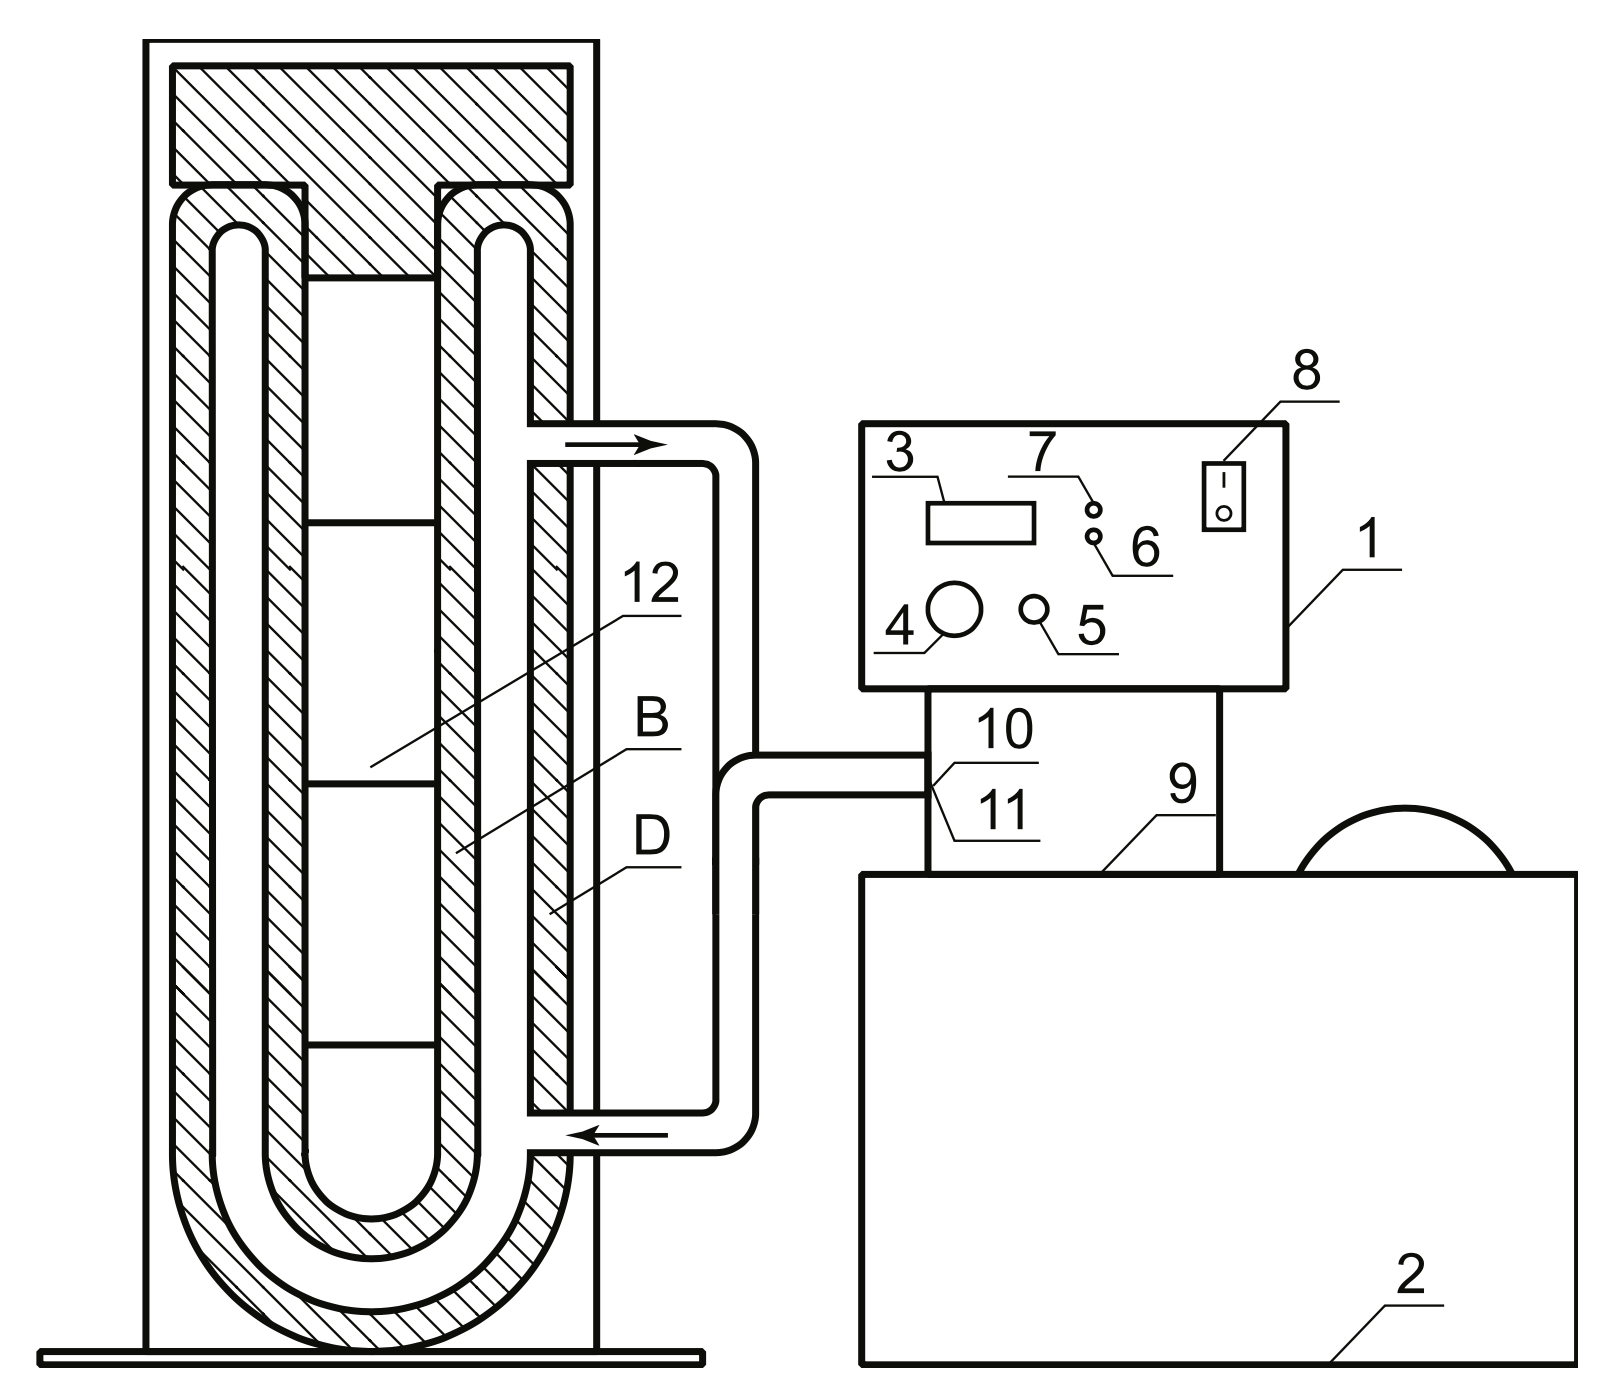
\includegraphics[scale = 0.3]{setup.png}
	\caption{Установка для определения коэффициента вязкости жидкости}
	\label{fig:setup}
\end{figure}

Сосуд помещён в термостат с циркуляцией воды для поддержания постоянной температуры. Температура жидкости контролируется термостатом с точностью до $\pm 0.1$°C. Измерения проводятся при различных температурах от комнатной до 50–60°C.

Радиусы шариков измеряются с помощью горизонтального компаратора или микроскопа. Для каждого шарика вычисляется среднее значение диаметра. Плотность шариков определяется по справочным таблицам, а плотность исследуемой жидкости — по графику зависимости $\rho_{ж}(T)$.

Термостат оборудован цифровым индикатором температуры, системой циркуляции жидкости и нагревателем. Регулировка температуры осуществляется с помощью ручки настройки. Включение нагрева и достижение установленной температуры сопровождаются светодиодными индикаторами.

Схема устройства термостата изображена на рисунке (\ref{fig:thermostat}).

\begin{figure}[h!]
	\centering
	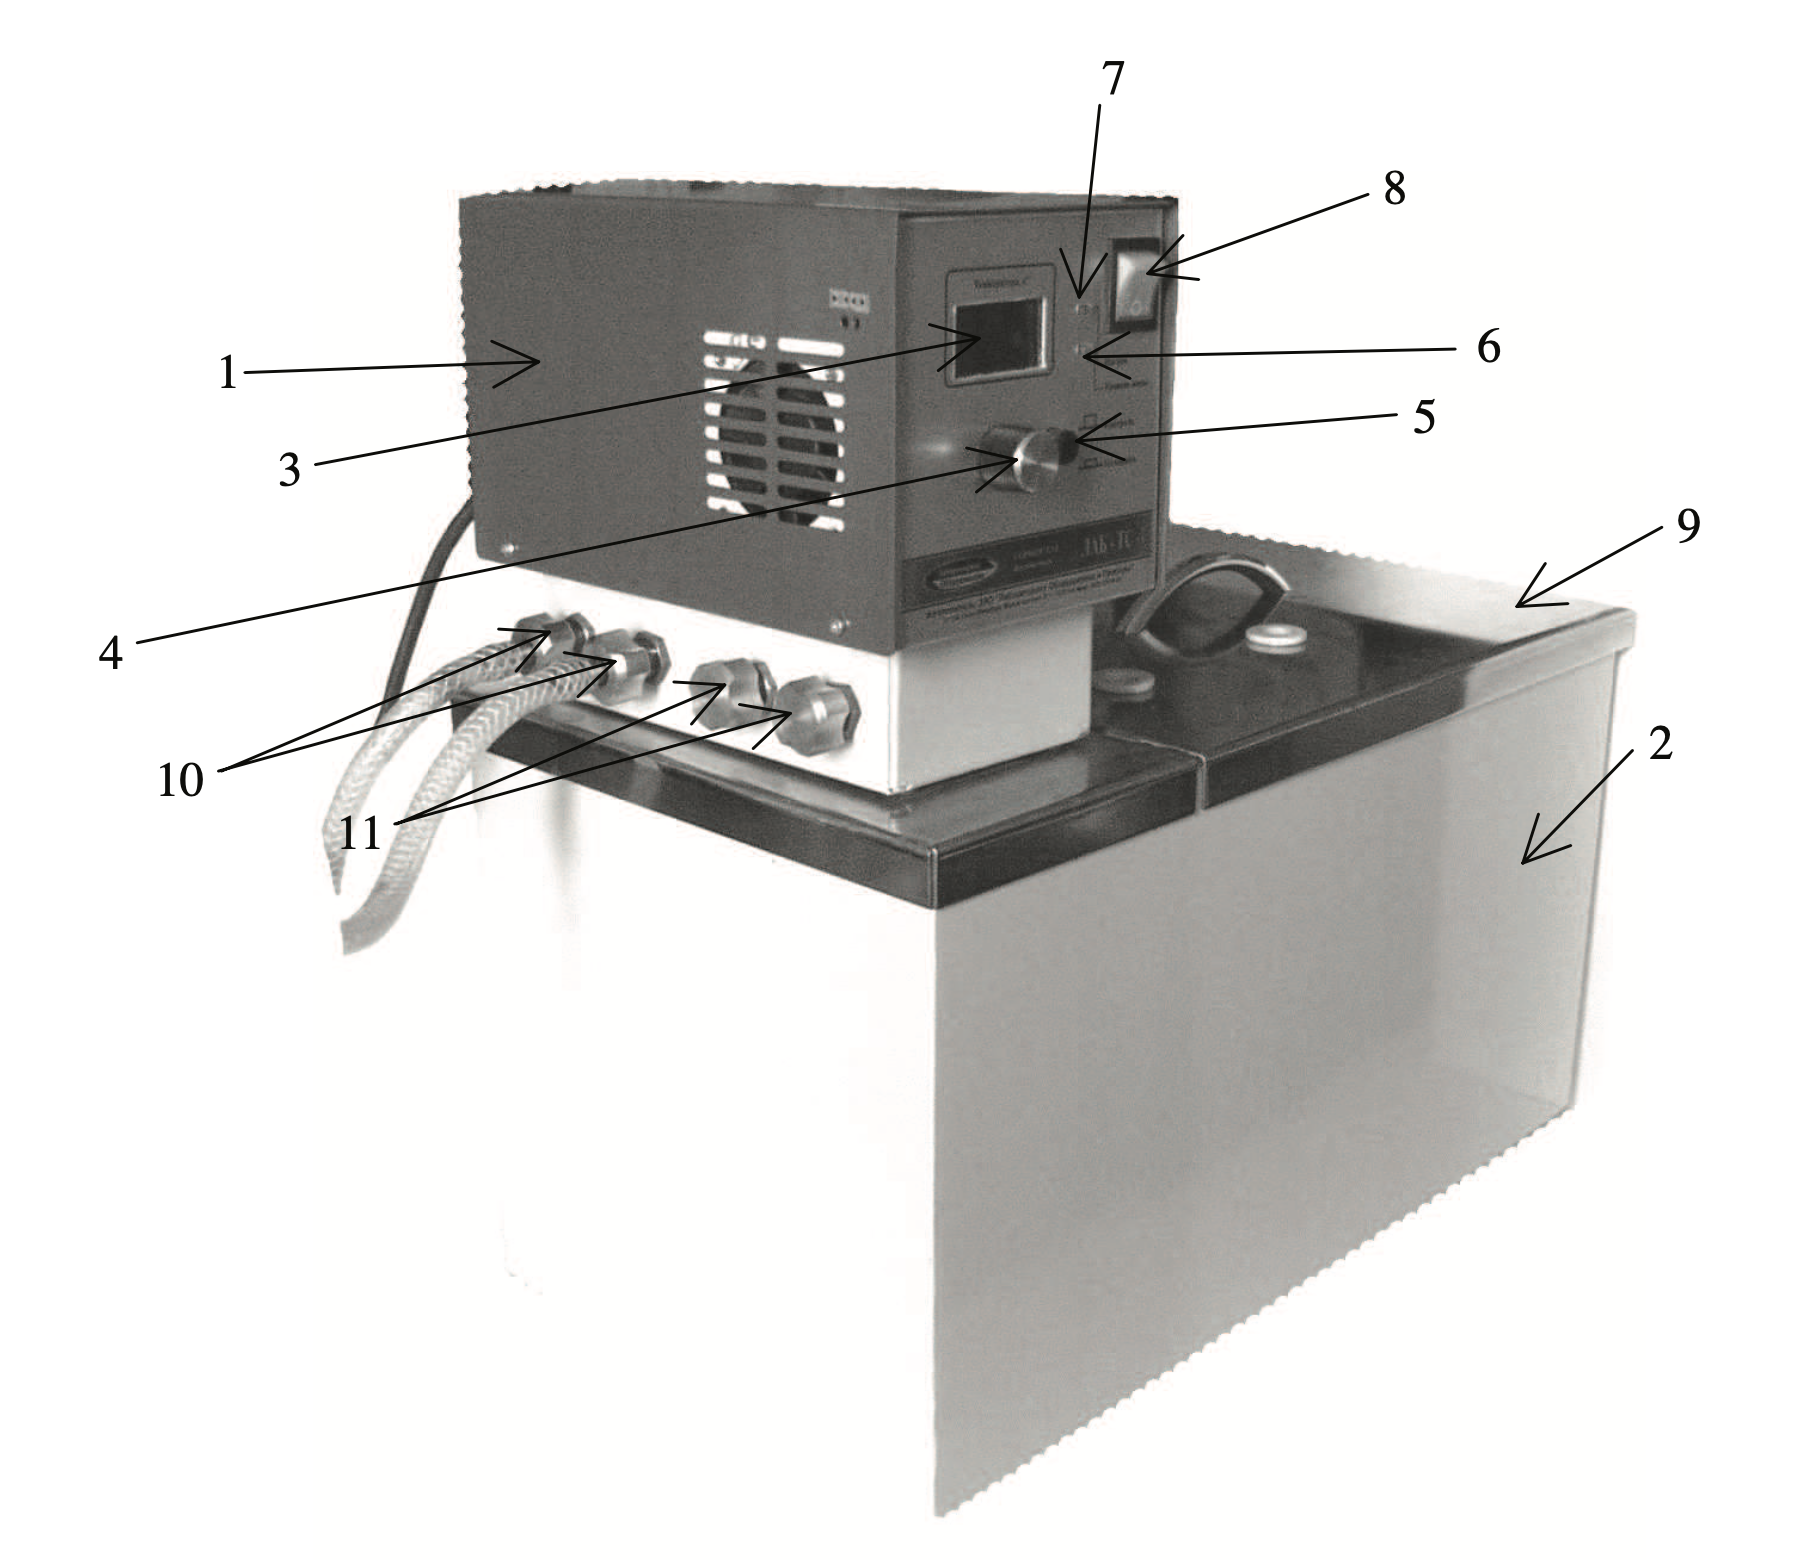
\includegraphics[scale = 0.3]{thermostat.png}
	\caption{Устройство термостата}
	\label{fig:thermostat}
\end{figure}

Опыт по измерению скорости падения шариков проводится после установления термического равновесия системы. Для каждого значения температуры выполняются несколько измерений с шариками различного диаметра.


\section*{Ход работы}

\begin{enumerate}
  \item Отберём $15-20$ шариков различного размера и с помощью компаратора или микроскопа измерим их средние диаметры.
  
  \item Измерим установившиеся скорости падения шариков и вычислите вязкость $\eta$ по формуле (\ref{eta}). Измерения выполним для $4-5$ значений температуры в интервале от комнатной до $50-60 ^\circ C$. Для каждого значения температуры определим плотность жидкости $\rho_\text{ж}$ по графику $\rho_\text{ж} (T)$, изображенного на рисунке (\ref{fig:rho_T}).
  
	\begin{figure}[h!]
		\centering
		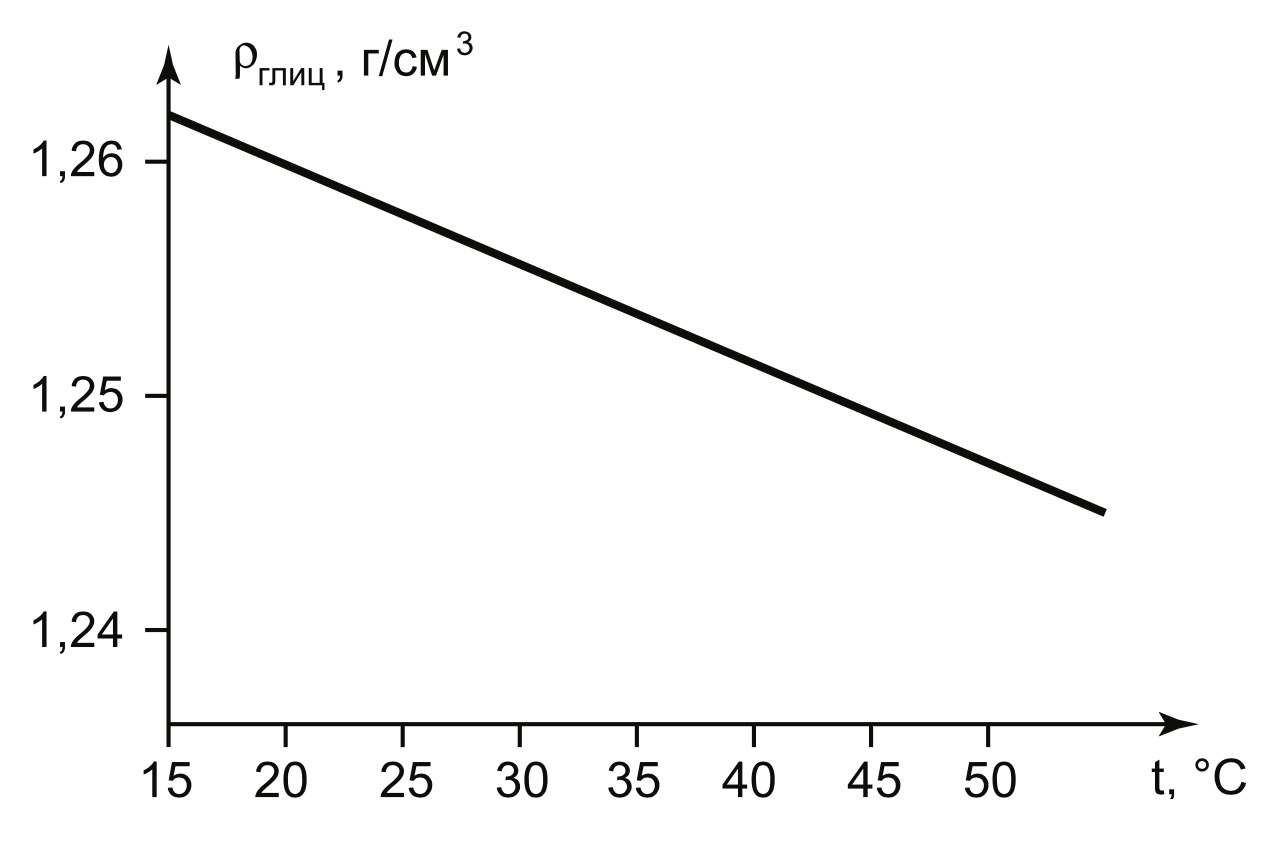
\includegraphics[scale = 0.35]{rho_t.png}
		\caption{Зависимость плотности глицерина от температуры}
		\label{fig:rho_T}
	\end{figure}
  
  \item Для каждого из опытов вычислим значение числа Рейнольдса $Re$, оценим время релаксации $\tau$ (по формуле (\ref{relax})) и путь релаксации $S = v_\text{уст} \tau$. Проанализируем применимость формулы Стокса в каждом эксперименте.
  
  \item Построим график зависимости $\ln \eta$ от $1/T$.
  
  \item По угловому коэффициенту прямой $\ln \eta (1/T)$ с помощью формулы (\ref{???}) определим энергию активации. 
  
	\item Оценим погрешность полученных результатов.
\end{enumerate}

\section*{Вывод}

Все цели работы были достигнуты.

\begin{enumerate}
	\item 
\end{enumerate}

\end{document}
